\documentclass{article}
\usepackage{graphicx}
\usepackage{enumerate}
\usepackage[margin=1in]{geometry}
\graphicspath{ {images/} }
\begin{document}

\section {The Basic HTTP GET / Response Questions}
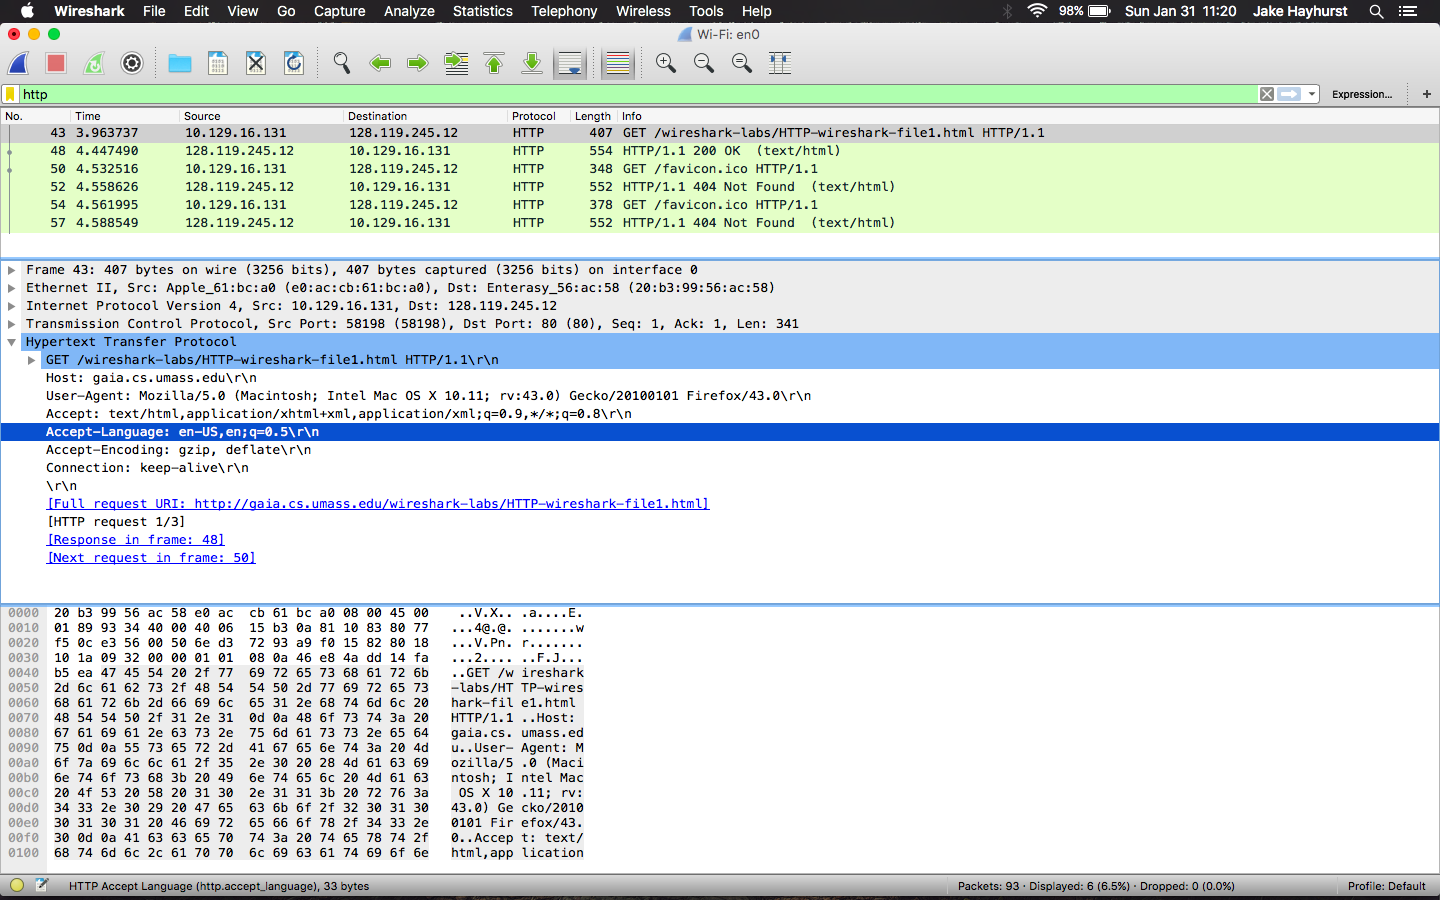
\includegraphics[width=\textwidth]{SimpleHTTPGet}\\
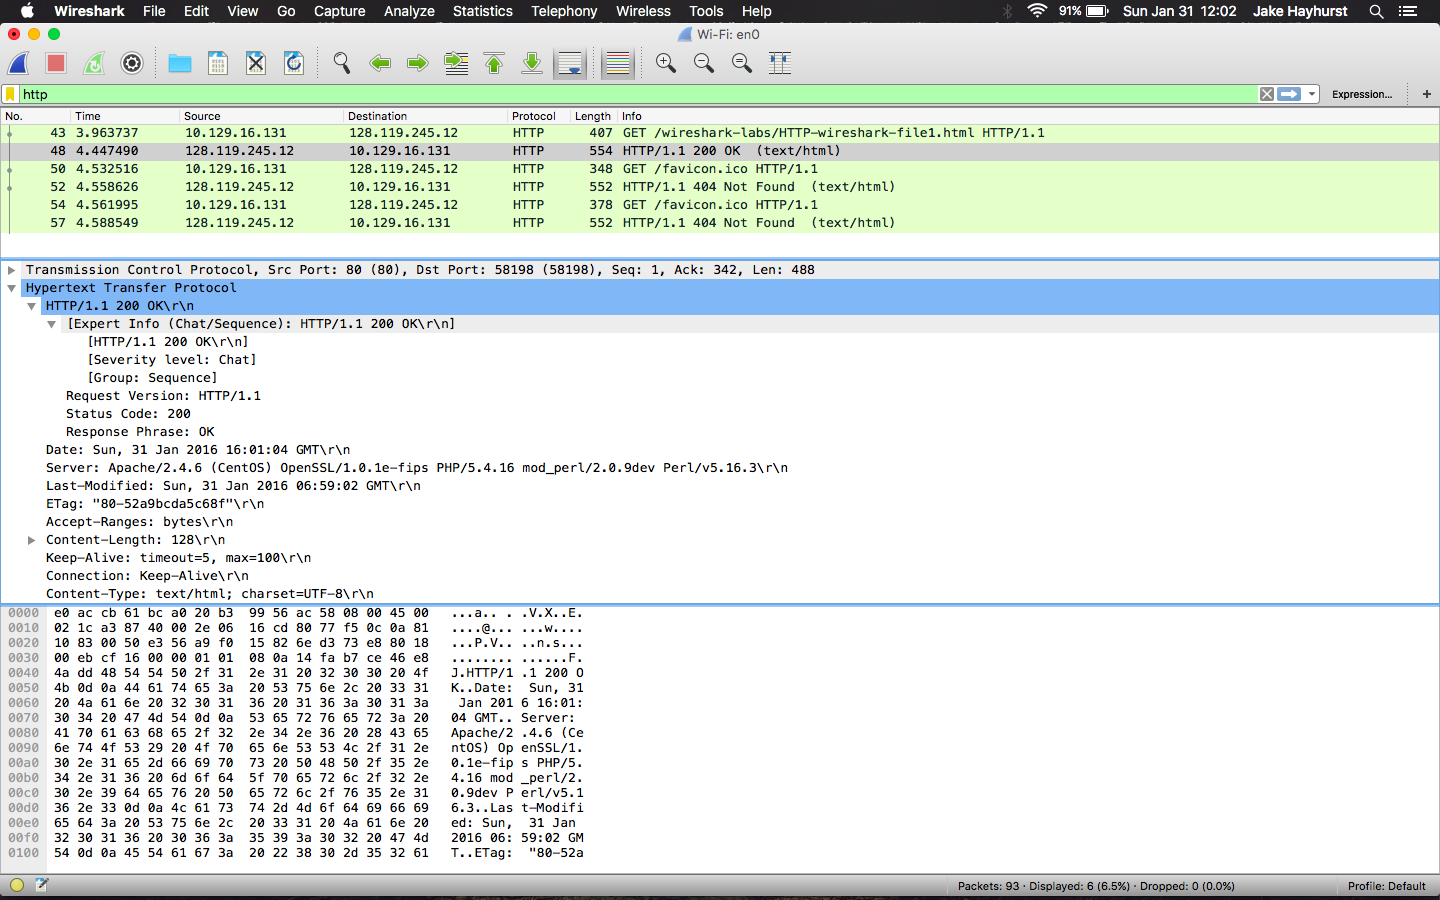
\includegraphics[width=\textwidth]{SimpleHTTPOk}\\\\
\begin{itemize}
  \item The browser is running HTTP version 1.1, this can be seen in the GET request in HTTP 1.1; The server is running HTTP 1.1 as the OK response is HTTP 1.1
  \item The languages that the browser indicate that it can accept en-US or just english text
  \item The IP address of my computer is 10.129.16.131, this is indicated by the source of the HTTP get request; The IP address of the web server is 128.119.245.12, this is indicated by the destination of the HTTP get request
  \item The status code returned from the server to the browser is 200, this is seen in the OK response from the server
  \item The HTML file was last modified on Sunday 31st January 2016 at 6:59:02 GMT this is seen in the HTTP OK response
  \item The total number of bytes being sent to the computer are 128, this can be seen in the HTTP OK response
  \item By inspecting the raw data displayed in the packet-listing window I did not see any additional headers
\end{itemize}

\section {The HTTP Conditional Get / Response Questions}
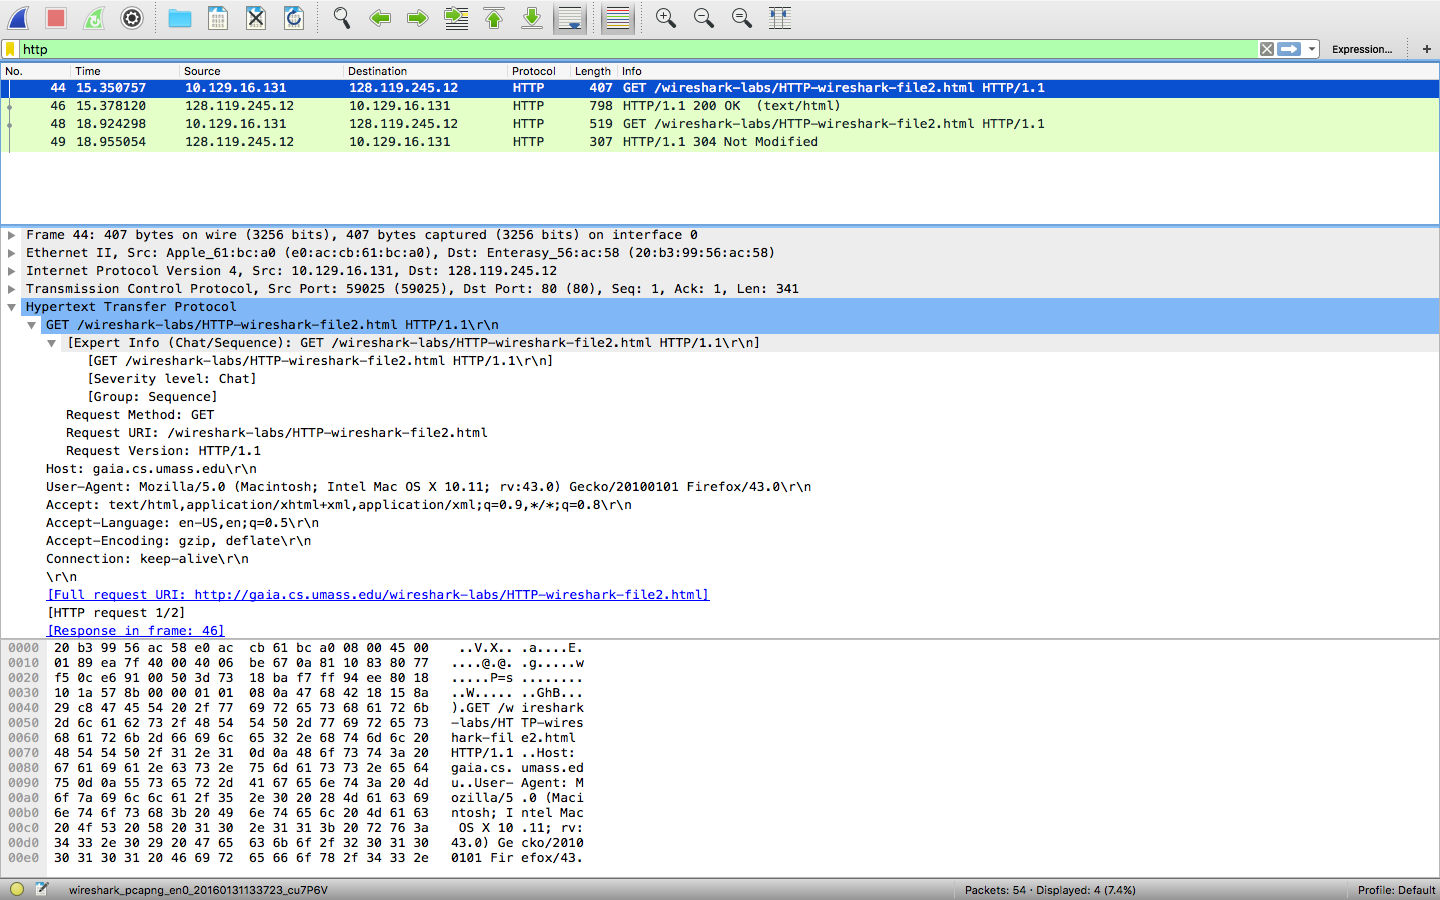
\includegraphics[width=\textwidth]{HTTPConditionalGet}\\
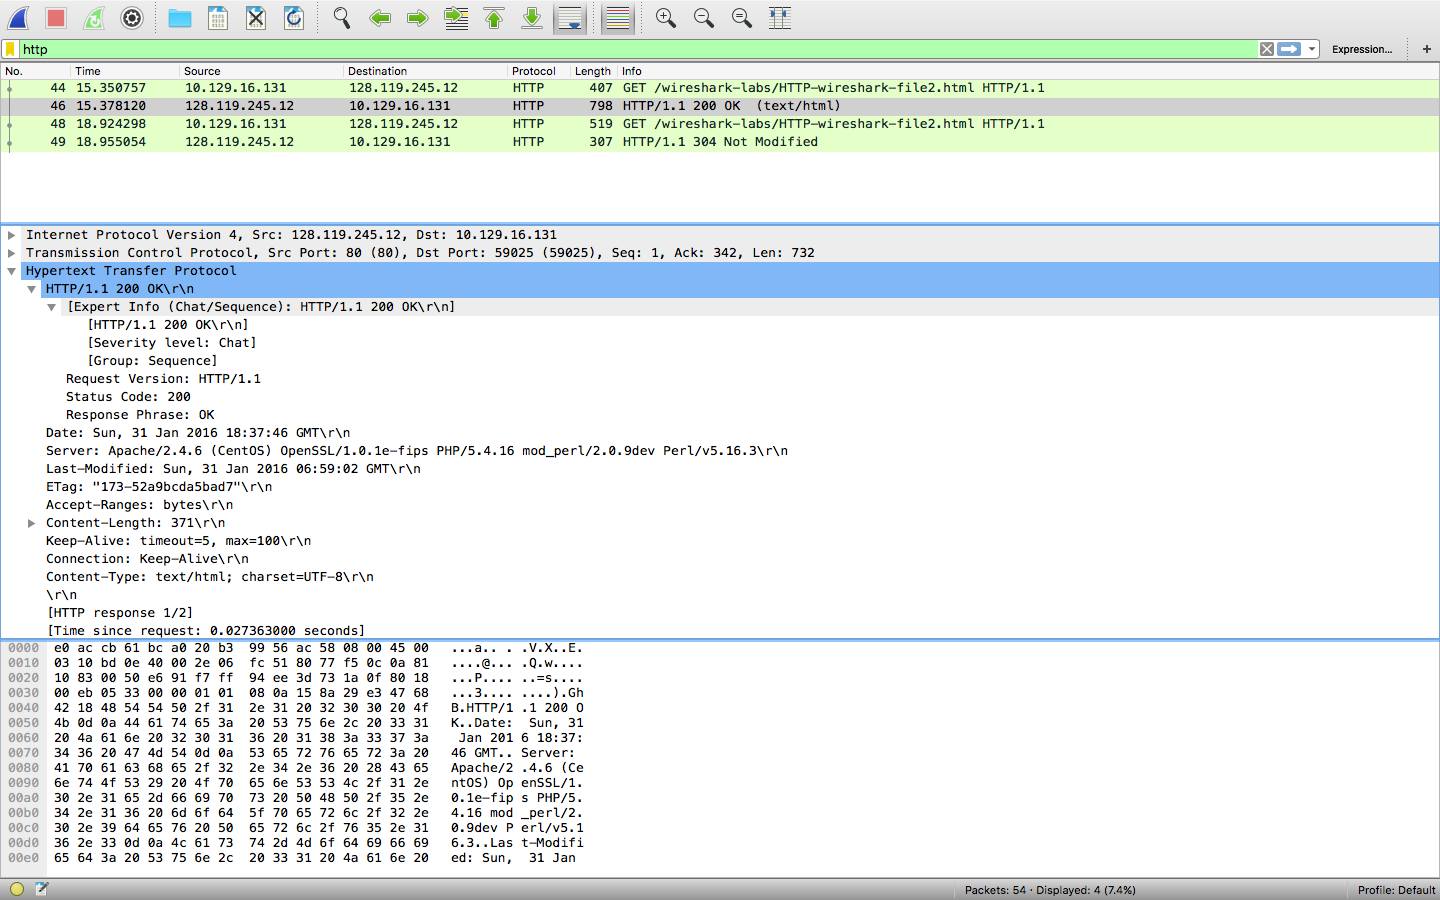
\includegraphics[width=\textwidth]{HTTPConditionalOk}\\
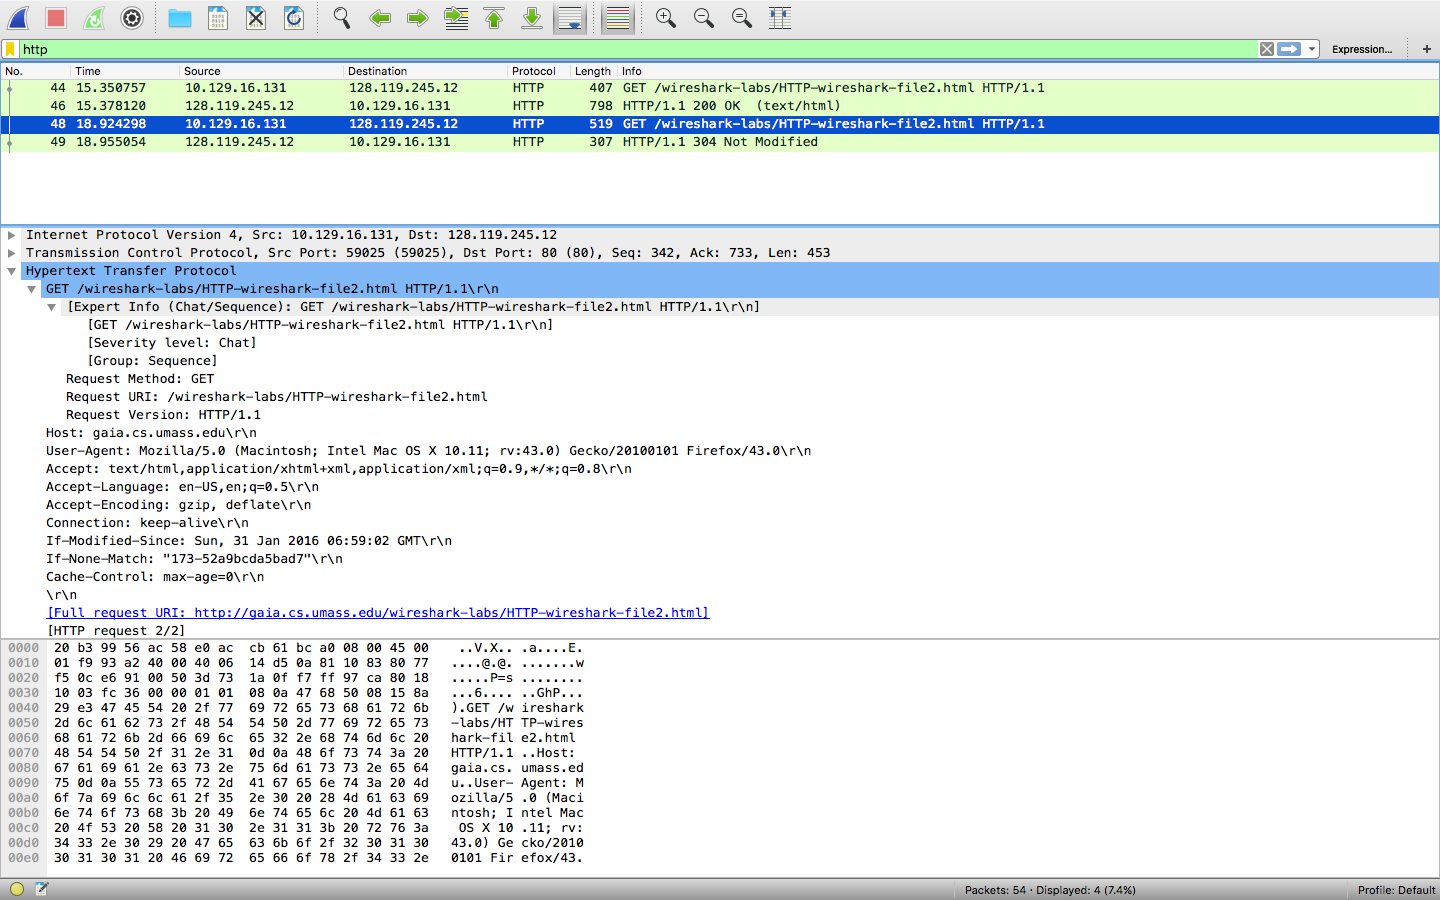
\includegraphics[width=\textwidth]{HTTPConditional2Get}\\
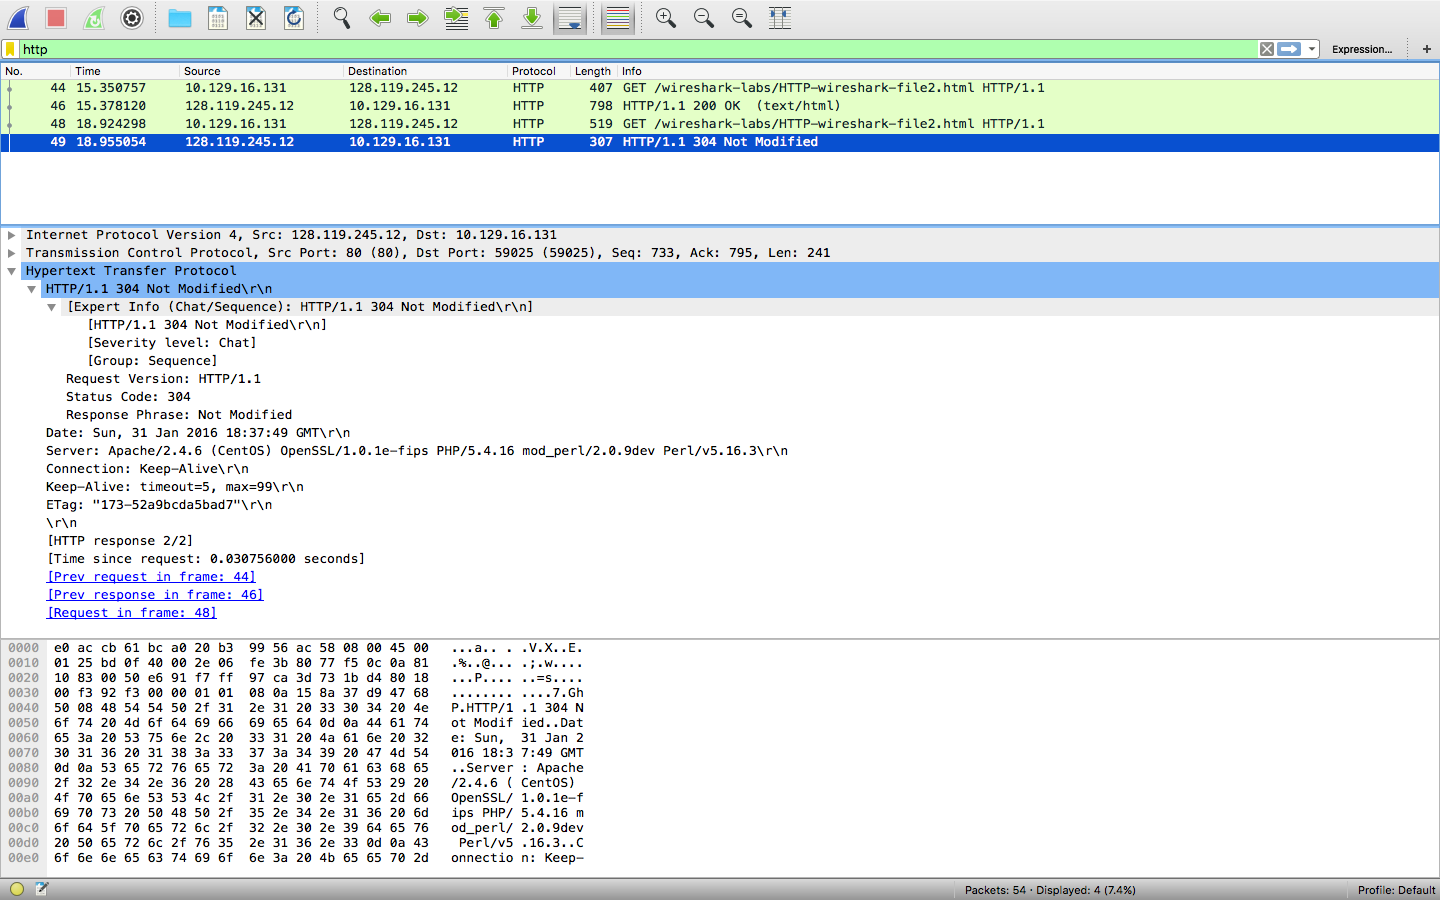
\includegraphics[width=\textwidth]{HTTPConditionalNotModified}\\
\begin{itemize}
  \item In the first contents of the HTTP GET request from the browser there is not an IF-MODIFIED-SINCE line in the packet
  \item The server explicitly returned a file, this can be seen in the HTTP OK response since the server sent a packet of length 371 bytes
  \item The second contents of the HTTP GET request from the browser there is an IF-MODIFIED-SINCE line in the packet. The information that follows the IF-MODIFIED-SINCE header is : Sun, 31 Jan 2016 06:59:02 GMT
  \item The status code and phrase of the response to the second HTTP Get is 304 Not Modified. The server did not explicitly return the contents of the file as it did not send anything other than header information in the packet
\end{itemize}

\section {Retrieving Long Documents Questions}
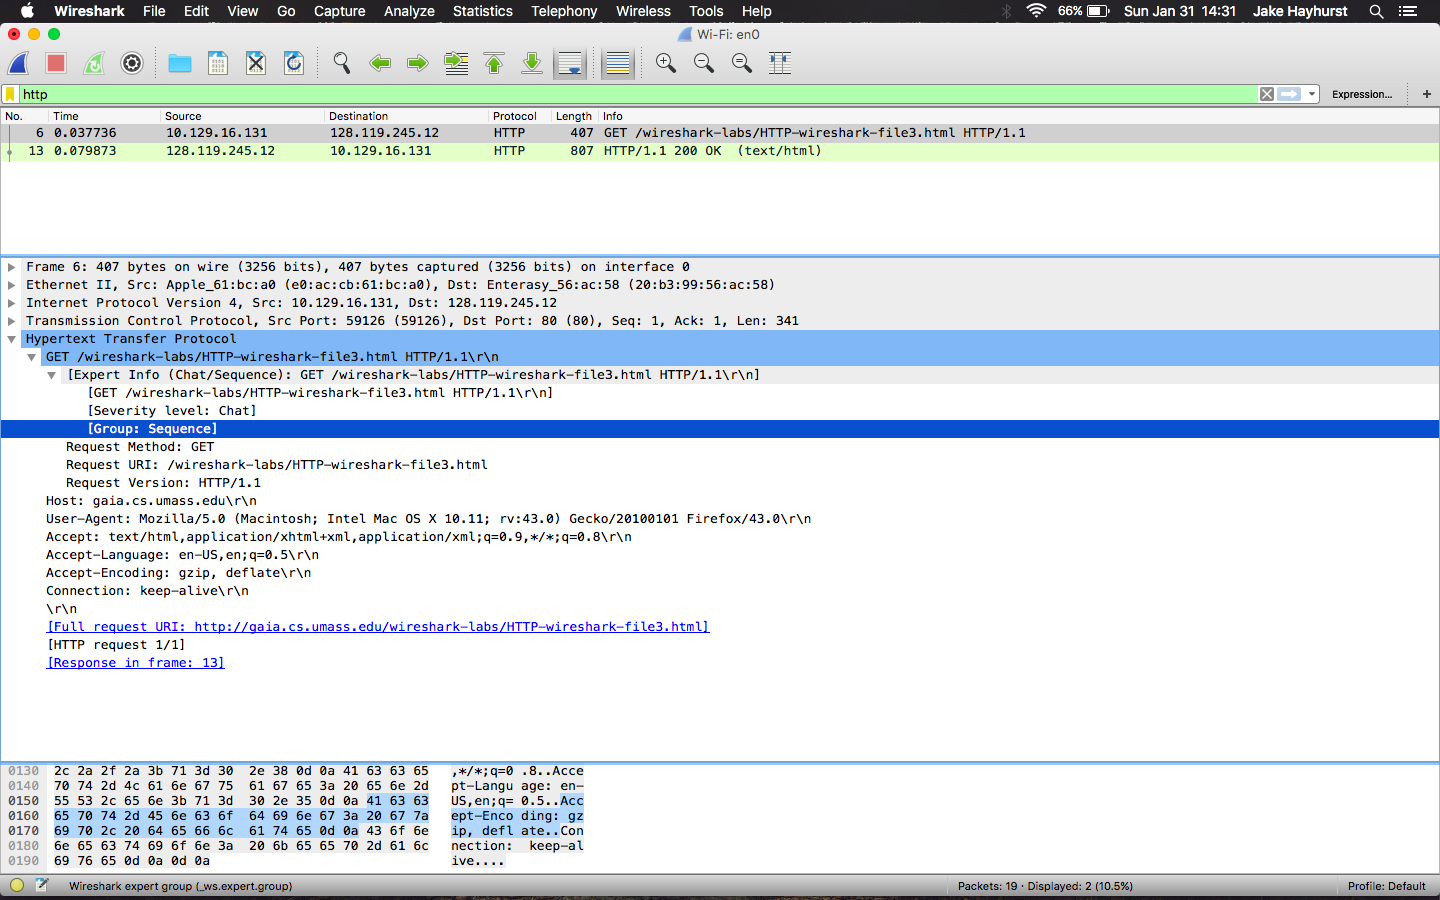
\includegraphics[width=\textwidth]{RetrievingLongDocumentsGet}\\
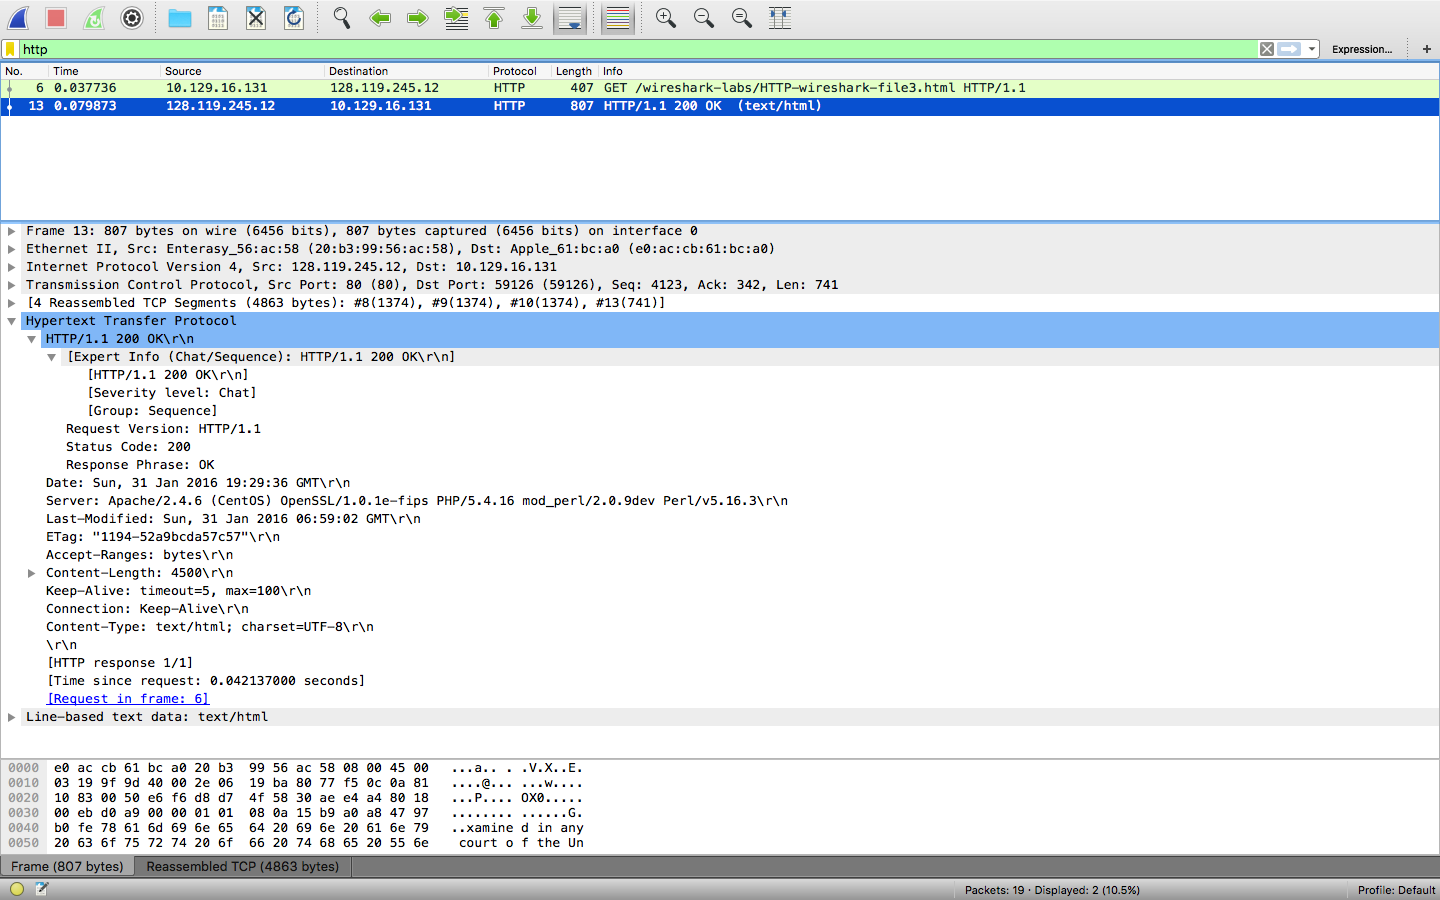
\includegraphics[width=\textwidth]{RetrievingLongDocumentsOk}\\
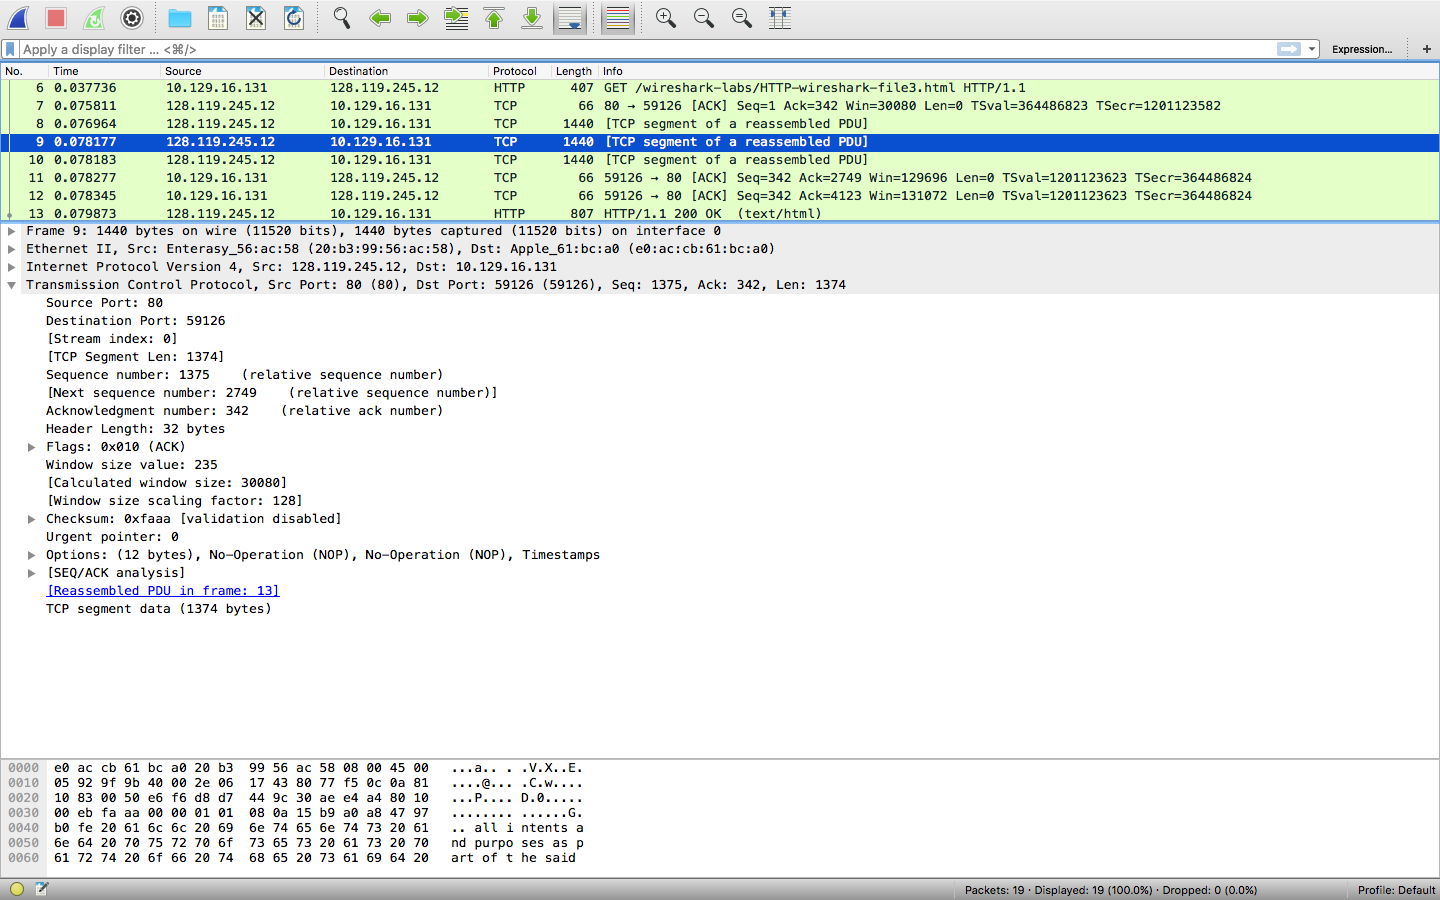
\includegraphics[width=\textwidth]{RetrievingLongDocumentsTCP}\\
\begin{itemize}
  \item The browser only sent one HTTP GET request. The packet number that contains the GET message is 6.
  \item The packet number that contains the status code and trace for the HTTP GET request was 13
  \item The status code and phrase in the HTTP GET response was 200 OK
  \item The amount of TCP segments needed to carry the single HTTP response and the text of the bill of rights were 3 segments at 1374 bytes per TCP segment
\end{itemize}

\section {HTML Documents with Embedded Objects Questions}
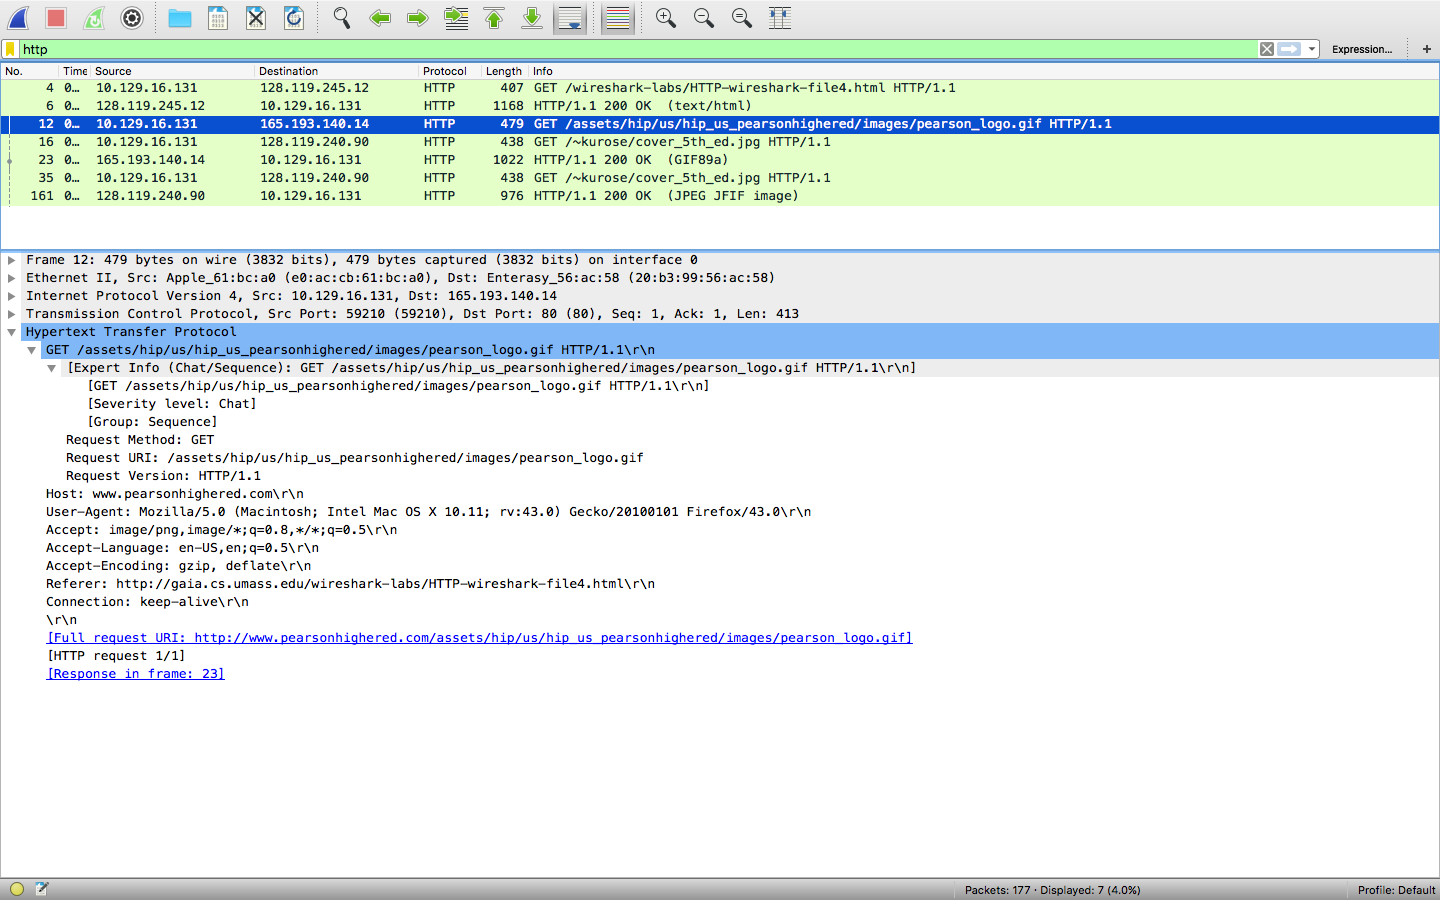
\includegraphics[width=\textwidth]{HTMLDocumentsWithEmbeddedObjectsGetGif}\\
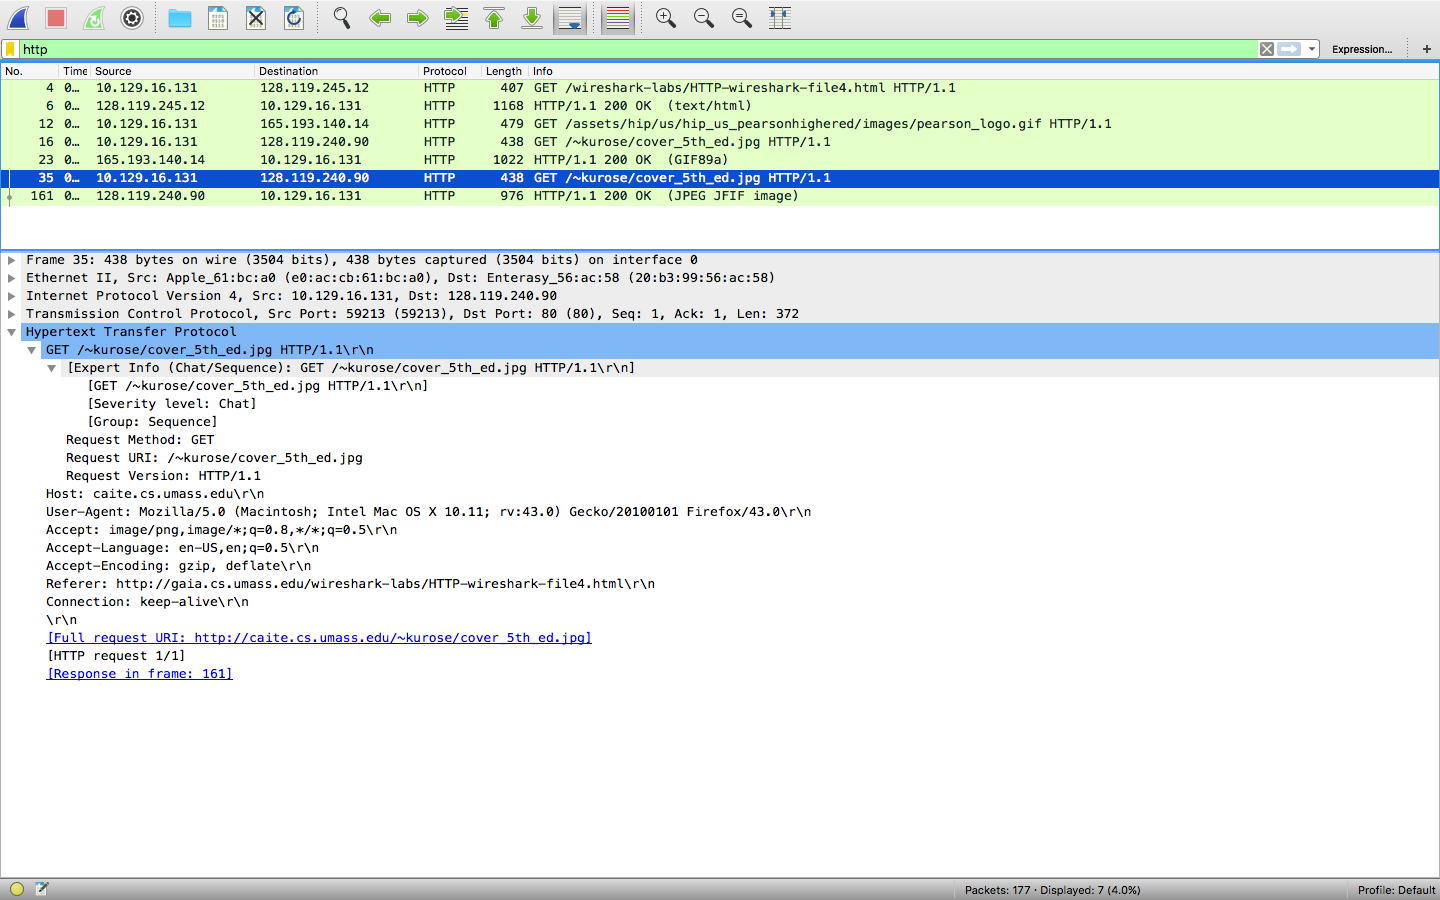
\includegraphics[width=\textwidth]{HTMLDocumentsWithEmbeddedObjectsGetJPG}\\\\
\begin{itemize}
  \item There were a total of 4 HTTP GET requests from the browser. These Get requests were to gaia.cs.umass.edu, www.pearsonhighered.com, manic.cs.umass.edu/, caite.cs.umass.edu/
  \item The browser appeared to download the images in parallel as there were two GET requests and then a response from the server
\end{itemize}

\section {HTTP Authentication Questions}
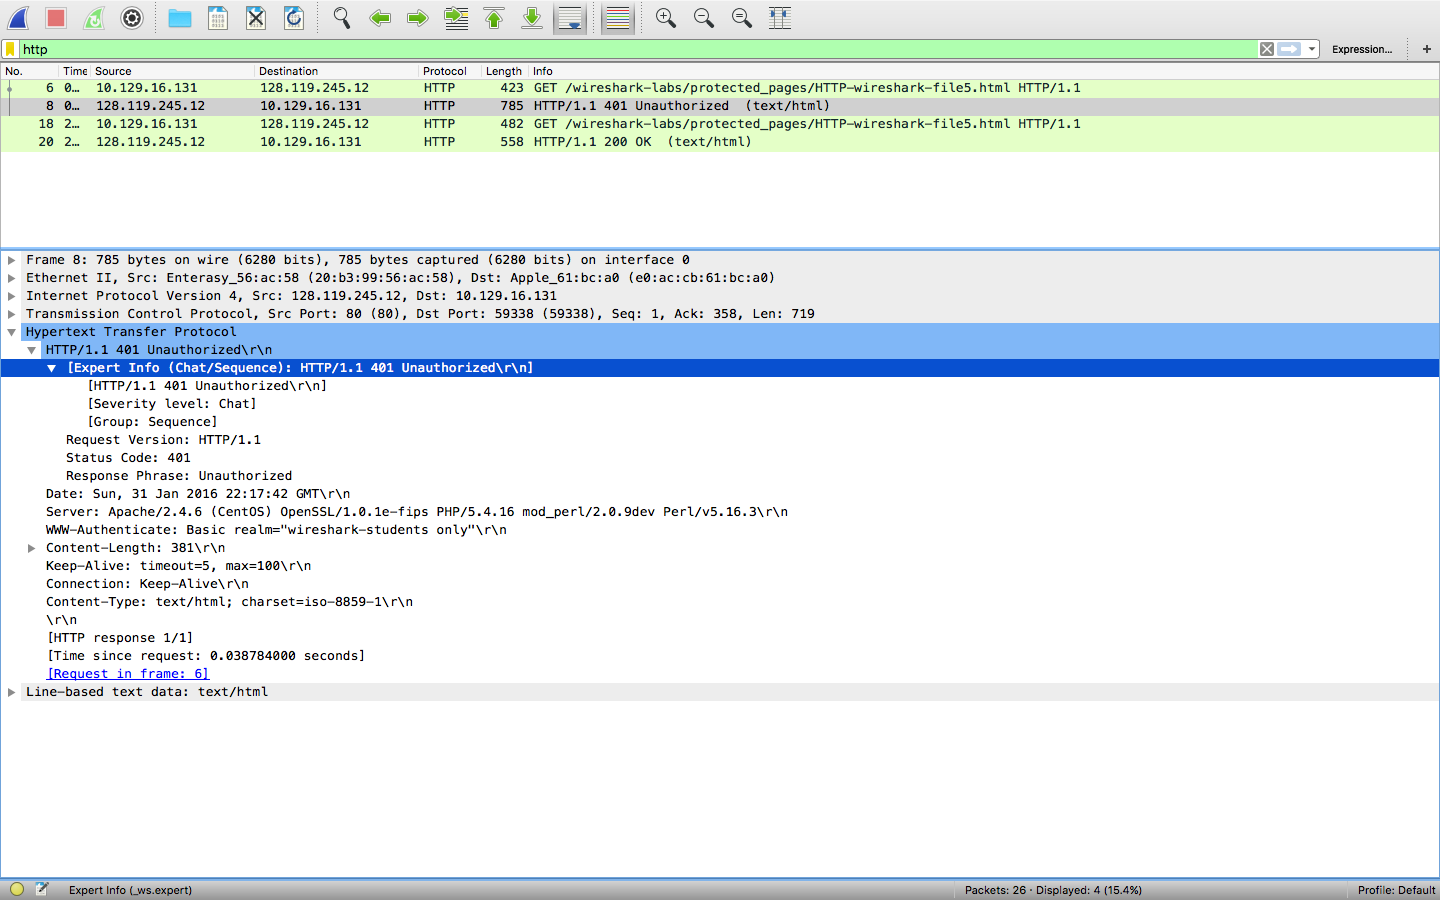
\includegraphics[width=\textwidth]{HTTPAuthenticationReply}\\
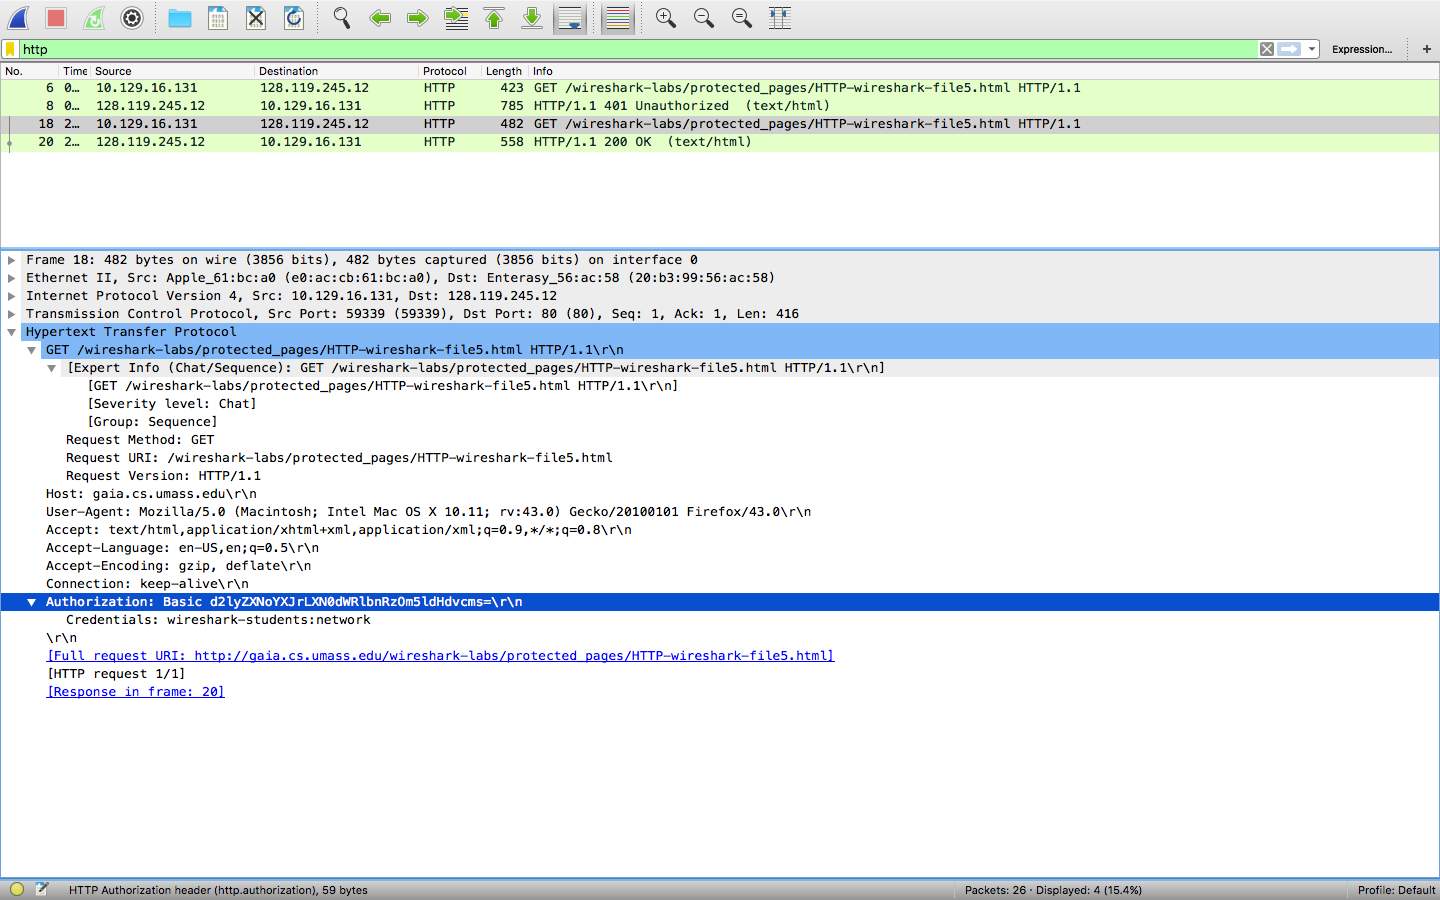
\includegraphics[width=\textwidth]{HTTPAuthenticationGet}\\
\begin{itemize}
  \item The servers response to the first HTTP GET is 401 Unauthorized
  \item With the second HTTP GET request from the browser the new field in the message is Authorization with the username and password displayed
\end{itemize}
\end{document}
